\documentclass[12pt]{article}% Your documentclass. I recommend something from the KOMA script class

%------------------------------------------%
%                Packages 
%------------------------------------------%
%------------------------------------------%
%                Packages
%------------------------------------------%

%------------------------------------------%
% Text encoding and layout
%------------------------------------------%

\usepackage[utf8]{inputenx}     % Proper input encoding (UTF-8)
\usepackage{ragged2e}           % Improved text alignment tools
\usepackage{setspace}           % Control line spacing (single, double, etc.)
\usepackage[
  paperwidth=8.5in,
  paperheight=11in,
  margin=1in
]{geometry}                     % Page dimensions and margins

%------------------------------------------%
% Graphics and float control
%------------------------------------------%

\usepackage{graphicx}           % Include graphics
\usepackage{grffile}            % Support graphics with multiple dots in filename
\usepackage{float}              % Improved float placement control
\usepackage{morefloats}         % Increase number of allowed floats
\usepackage{placeins}           % \FloatBarrier to keep floats within sections
\usepackage{pdflscape}          % Landscape pages in PDF
\usepackage{everypage}          % Page number control for rotated pages

%------------------------------------------%
% Mathematics
%------------------------------------------%

\usepackage{amsmath, amssymb, mathrsfs,bbold} % Core math packages
\usepackage{bm}                        % Bold math symbols
\usepackage{accents}                   % Custom math accents

%------------------------------------------%
% Tables
%------------------------------------------%

\usepackage{booktabs}        % Professional-quality tables
\usepackage{threeparttable}  % Tables with notes below
\usepackage{rotating}        % Sideways tables
\usepackage{adjustbox}       % Resize tables/figures relative to text width
\usepackage{siunitx}         % Align numbers by decimal; handle units
\usepackage{longtable}       % Multi-page tables (kableExtra longtable output)
\usepackage{multirow}        % Multi-row cells (kableExtra collapse_rows)
\usepackage{makecell}        % Line breaks inside cells

\sisetup{
  detect-mode,
  group-digits           = false,
  input-symbols          = {( ) [ ] - +},
  table-align-text-post  = false,
  input-signs            = ,
  separate-uncertainty   = true
}

%------------------------------------------%
% Captions and subfigures
%------------------------------------------%

\usepackage{caption}
\usepackage[list=true]{subcaption}
\captionsetup[table]{position=top}
\captionsetup[figure]{position=bottom}

%------------------------------------------%
% Colors and text utilities
%------------------------------------------%

\usepackage{xcolor}     % Extended color support
\usepackage{soul}       % Highlighting and letter spacing
\usepackage{comment}    % Block comments

%------------------------------------------%
% Appendix formatting
%------------------------------------------%

\usepackage[titletoc]{appendix}  % Appendix control and ToC integration

%------------------------------------------%
% Bibliography
%------------------------------------------%

\usepackage{natbib}     % Author-year citation management

%------------------------------------------%
% Hyperlinks (load near the end)
%------------------------------------------%

\usepackage[
  breaklinks,
  colorlinks,
  linkcolor=black,
  citecolor=black,
  urlcolor=blue,
  hyperfootnotes=false
]{hyperref}

% Allow URL line breaks at many characters
\def\UrlBreaks{%
\do\/\do-\do.\do=\do_\do?\do\&\do\%\do\a\do\b\do\c\do\d\do\e\do\f\do\g\do\h%
\do\i\do\j\do\k\do\l\do\m\do\n\do\o\do\p\do\q\do\r\do\s\do\t\do\u\do\v\do\w%
\do\x\do\y\do\z\do\A\do\B\do\C\do\D\do\E\do\F\do\G\do\H\do\I\do\J\do\K\do\L%
\do\M\do\N\do\O\do\P\do\Q\do\R\do\S\do\T\do\U\do\V\do\W\do\X\do\Y\do\Z%
\do\0\do\1\do\2\do\3\do\4\do\5\do\6\do\7\do\8\do\9}

%------------------------------------------%
%              Custom Commands 
%------------------------------------------%
%These are the custom commands that I use in the latex document

\newcommand\iid{i.i.d.} %Makes iid a command
\newcommand\pN{\mathcal{N}} %Makes the natural numbers a command


\setcounter{MaxMatrixCols}{20}

\newtheorem{theorem}{Theorem}%[section]
\newtheorem{lemma}[theorem]{Lemma}
\newtheorem{proposition}[theorem]{Proposition}
\newtheorem{corollary}[theorem]{Corollary}
\newtheorem{assumption}[theorem]{Assumption}
\newenvironment{proof}{\paragraph{Proof:}}{\hfill$\square$ \\} %This fixes the problem with dynamic tables for some reason

%For Page Numbers while rotated
\newlength{\hfoot}
\newlength{\vfoot}
\AddEverypageHook{\ifdim\textwidth=\linewidth\relax
\else\setlength{\hfoot}{-\topmargin}%
\addtolength{\hfoot}{-\headheight}%
\addtolength{\hfoot}{-\headsep}%
\addtolength{\hfoot}{-.5\linewidth}%
\ifodd\value{page}\setlength{\vfoot}{\oddsidemargin}%
\else\setlength{\vfoot}{\evensidemargin}\fi%
\addtolength{\vfoot}{\textheight}%
\addtolength{\vfoot}{\footskip}%
\raisebox{\hfoot}[0pt][0pt]{\rlap{\hspace{\vfoot}\rotatebox[origin=cB]{90}{\thepage}}}\fi}
%http://tex.stackexchange.com/questions/209685/landscape-mode-and-page-numbering

%------------------------------------------%
%      Matter Related to Table Creation 
%------------------------------------------%
%This helps with custom automatic tables. It uses latex  functions
%http://www.jwe.cc/2012/03/stata-latex-tables-estout/
%http://repec.org/bocode/e/estout/estout.html

% *****************************************************************
% Estout related things
% *****************************************************************
\let\estinput=\input % define a new input command so that we can still flatten the document

\newcommand{\estwide}[3]{
    \vspace{.75ex}{
      \textsymbols% Note the added command here
      \begin{tabular*}
      {\textwidth}{@{\hskip\tabcolsep\extracolsep\fill}l*{#2}{#3}}
      \toprule
      \estinput{#1}
      \bottomrule
      \addlinespace[.75ex]
      \end{tabular*}
      }
    } 

\newcommand{\estauto}[3]{
    \vspace{.75ex}{
      \textsymbols% Note the added command here
      \begin{tabular}{l*{#2}{#3}}
      \toprule
      \estinput{#1}
      \bottomrule
      \addlinespace[.75ex]
      \end{tabular}
      }
    }

% Allow line breaks with \\ in specialcells
\newcommand{\specialcell}[2][c]{%
    \begin{tabular}[#1]{@{}c@{}}#2\end{tabular}
}
\DeclareUnicodeCharacter{00A0}{ }
% *****************************************************************
% Custom subcaptions
% *****************************************************************
% Note/Source/Text after Tables
% The new approach using threeparttables to generate notes that are the exact width of the table.
\newcommand{\Figtext}[1]{%
  \begin{tablenotes}[para,flushleft]
  \hspace{6pt}
  \hangindent=1.75em
  #1
  \end{tablenotes}
  }
\newcommand{\Fignote}[1]{\Figtext{\emph{Note:~}~#1}}
\newcommand{\Figsource}[1]{\Figtext{\emph{Source:~}~#1}}
\newcommand{\Starnote}{\Figtext{* p $<$ 0.1, ** p $<$ 0.05, *** p $<$ 0.01. Robust standard errors in parentheses.}}% Add significance note with \starnote
% If you are using hyper-ref (recommended), this command must go after all 
% other package inclusions (from the hyperref package documentation).
% The purpose of hyperref is to make the PDF created extensively
% cross-referenced.

\newcommand{\sym}[1]{\rlap{#1}} %Allows for fancy stars in tables that also works in beamer

% Create a function that works for the non-linear symbols
\newcommand{\nlsym}[1]{\rlap{\append{}{*}{#1}}} %Allows for fancy stars in tables that also works in beamer

% Character substitution that prints brackets and the minus symbol in text mode. Thanks to David Carlisle
\def\yyy{%
  \bgroup\uccode`\~\expandafter`\string-%
  \uppercase{\egroup\edef~{\noexpand\text{\llap{\textendash}\relax}}}%
  \mathcode\expandafter`\string-"8000 }

\def\xxxl#1{%
\bgroup\uccode`\~\expandafter`\string#1%
\uppercase{\egroup\edef~{\noexpand\text{\noexpand\llap{\string#1}}}}%
\mathcode\expandafter`\string#1"8000 }

\def\xxxr#1{%
\bgroup\uccode`\~\expandafter`\string#1%
\uppercase{\egroup\edef~{\noexpand\text{\noexpand\rlap{\string#1}}}}%
\mathcode\expandafter`\string#1"8000 }

\def\textsymbols{\xxxl[\xxxr]\xxxl(\xxxr)\yyy}


%Protects against odd minus sign errors within the tables
\catcode`_11
\protected\def \c__siunitx_minus_tl {$-$}
\catcode`_ 8 

%-----------Tables-------------%
% This Section is needed to make the tables work with amsmath. But because of the \( being open and having no match, Sublime Text thinks that everything after it (all text) is in math mode and hence changes the text color. This annoys me so the only ``solution'' is to just place this preamble here. It seems to work still. 
\makeatletter 
\edef\originalbmathcode{%
    \noexpand\mathchardef\noexpand\@tempa\the\mathcode`\(\relax} %\)

\def\resetMathstrut@{%
  \setbox\z@\hbox{%
    \originalbmathcode

    \def\@tempb##1"##2##3{\the\textfont"##3\char"}%
    \expandafter\@tempb\meaning\@tempa \relax
  }%
  \ht\Mathstrutbox@\ht\z@ \dp\Mathstrutbox@\dp\z@
}
\makeatother %./tables.tex:25: LaTeX Error: Bad math environment delimiter. [\)]
\usepackage{xparse}

\ExplSyntaxOn
\DeclareExpandableDocumentCommand{\append}{mmm}
 {
  #1\prg_replicate:nn{#3}{#2}
 }
\ExplSyntaxOff

\doublespacing

% Keep tables (body and notes) single-spaced despite the document's double spacing
\usepackage{etoolbox}
\AtBeginEnvironment{table}{\singlespacing}


  \begin{document}
%------------------------------------------%
%     Title Page
%------------------------------------------%

\begin{titlepage}
\vspace*{.25cm}
\begin{center}
\renewcommand{\thefootnote}{\fnsymbol{footnote}}
\textbf{
\noindent\LARGE
\title
~
The Socio-Economic Benefits of Hurricane Forecasting Augmented Observations (Final Report)
}

\vspace{.7cm}
%\vspace{.4cm}
{\Large Renato Molina, Ivan Rudik, Diego Cardoso, and Brian McNoldy.\footnote{Renato Molina (University of Miami), Ivan Rudik (Cornell University), Diego Cardoso (University of Illinois Urbana-Champaign), and Brian McNoldy (University of Miami). We thank Mark DeMaria, Sarah Ditchek and Jason Sippel for providing hurricane forecast model output.}} \\

\vspace{.25cm}
{\Large\today}\\
\vspace{.25cm}
\end{center}

\begin{abstract}
\begin{normalsize}
\begin{singlespace}
This study quantifies the socio-economic value of augmented aircraft observations in hurricane forecasting. By linking data-denial experiments for eight U.S. hurricane landfalls (2017–2020) to a structural model of hurricane costs, we isolate the economic returns of in-situ reconnaissance. We find that augmented observations reduce forecast uncertainty by 0.26 m/s at the 3-day lead time. Implementing this improvement into a valuation framework, this precision gain generates \$24 million in social value per affected county. The resulting magnitude implies a benefit-to-cost ratio, these findings provide support for the strategic recapitalization of the NOAA aircraft fleet.
\end{singlespace}
\end{normalsize}
\end{abstract}

%abstract

%\vspace{.6cm}

\noindent\textbf{JEL:} Q54, D81, D83, O33

\vspace{.6cm} 

\noindent\textbf{Keywords:} Value of Information, Hurricane Forecasting, Augmented Observations, Socio-economic Benefits.
\setcounter{footnote}{0}


\end{titlepage}

\newpage
%------------------------------------------%
%                Table of Contents
%------------------------------------------%

 \begin{singlespace}
 	\tableofcontents
 	\listoftables
 	\listoffigures
 \end{singlespace}
 \newpage

%------------------------------------------%
%                Main text
%------------------------------------------%
 \FloatBarrier
%------------------------------------------%
%                Introduction
%------------------------------------------%
\section{Introduction} \label{sec:intro}

The Atlantic hurricane season poses a perennial threat to the coastal United States, with landfalling tropical cyclones causing catastrophic economic losses and significant casualties. To mitigate these impacts, the National Oceanic and Atmospheric Administration (NOAA) and the National Hurricane Center (NHC) rely on a sophisticated infrastructure of observations and numerical modeling to forecast storm track and intensity. Among these observational tools, augmented aircraft reconnaissance, also known as \emph{augmented observations} (AO), provides high-resolution, in-situ atmospheric data that are critical for the accurate initialization of forecast models.

The meteorological value of these AO is well-documented through decades of ``data denial'' experiments. These experiments, which consist of running hurricane predictions with and without said AO, consistently demonstrate reductions in track and intensity errors \citep{Majumdar2016}. However, the \emph{socioeconomic} return on these investments remains less understood. Quantifying how improved forecast accuracy translates into tangible societal benefits, such as reduced capital losses and avoided fatalities, is essential for justifying the substantial costs associated with maintaining and modernizing AO's capabilities.

This report presents a comprehensive data-driven analysis of the socioeconomic benefits of augmented hurricane observations. Leveraging previous work on the social value of hurricane forecast \cite{molina2024social} and a high-fidelity dataset of data denial experiments derived from \citet{DitchekEA2023}, this study isolates the economic impact of aircraft reconnaissance for eight (Category 1 and above) landfalling hurricanes between 2017 and 2020, including Hurricanes Harvey, Irma, and Michael. We perform an estimation of the share of social value that can be attributed to augmented observation, document a replicable methodology for future estimations, and general policy recommendations for improved  benefit-cost assessments of these programs.

%------------------------------------------%
%      Institutional Background
%------------------------------------------%
\section{Institutional Background} \label{sec:background}

Hurricanes form and spend the majority of their lifetimes over the open ocean, where in-situ measurements are difficult and expensive to collect. To collect vital data in and around life-threatening hurricanes in the Atlantic, hurricane reconnaissance flights began in the mid-1940s, flown by the United States Navy and Air Force. By the mid-1950s, routine reconnaissance flights were also conducted by the United States Weather Bureau’s National Hurricane Research Project (NHRP), the precursor to what is now the Hurricane Research Division (HRD), operated by the National Oceanic and Atmospheric Administration (NOAA). HRD has been conducting operational and research flights into and around hurricanes since 1982, and the Air Force's history of flying into hurricanes began nearly four decades prior \citep{Sheets1990,Marks_Shay1998}.

However, not all hurricanes have reconnaissance flights into and around them. The National Hurricane Center (NHC) within NOAA is the primary decision-maker of what and when to fly \citep{OFCM2024,RappaportEA2009}. Specialists at NHC are tasked with identifying if a tropical cyclone has formed, how intense it is, how large it is, and other vital statistics. They are also tasked with forecasting a storm's future track and intensity, which is aided when aircraft reconnaissance data are provided to the forecast models. Priority for resources is given to proximity to land, potential for significant impacts on land, and challenging environmental conditions that increase forecast uncertainty \citep{Aberson2003, Majumdar2016}. Once a reconnaissance flight is requested, coordination between NHC, the U.S. Air Force, and HRD determines what planes will fly, where they will fly, and what instruments need to be available \citep{OFCM2024}.

Aside from flight-level measurements of wind speed, estimates of the storm's central pressure, and radar mapping of the storm's structure, a key instrument over the past four decades has been the dropwindsonde (often called a ``dropsonde"). This is an instrument package released from an aircraft that collects high-resolution in-situ data along a vertical profile of the atmosphere down to the ocean surface as it falls slowly with the aid of a parachute \citep{Hock_Franklin1999}.

These data are collected and processed by forecast models in real-time. In principle, providing more data to a model will improve its ability to accurately represent and forecast the atmosphere. This process is called data assimilation (DA) and it is a fundamental and complex step in all of numerical weather prediction \citep{Kalnay2003, Bannister2017}. Providing a hurricane model with information about the intensity, structure, and surrounding environment of the hurricane should, in general, make that model more accurate.

\subsection{Data Denial Experiments}

One of the earliest studies to document the impact of dropsonde observations on hurricane track forecast models was \citet{Franklin_DeMaria1992}. They utilized data from fourteen Atlantic hurricane surveillance flights spanning 1982-1989 and conducted data denial experiments in a research-grade model. In a data denial experiment, a model is run with and without a specific dataset, then the results are validated against the observations (``truth"), and relative improvements or degradations are calculated. In this case, when including dropsonde data, the overall reduction in track error was approximately 16\% in the critical 24-36-hour lead times, with a positive impact at all lead times.

\citet{BurpeeEA1996} provides the first robust accounting of a data denial study using an operational forecast model. This experiment utilized data from 28 Atlantic hurricane flights spanning 1982-1993 with a total of 686 dropsondes. In that seminal study, track errors were reduced by 16-30\% in the 12-60-hour lead times by including the dropsonde data, a feat the authors appropriately called a ``breakthrough".

HRD acquired a Gulfstream-IV high-altitude aircraft in 1997 and that has been utilized for hurricane surveillance flights to this day. Some of the earlier data-denial studies were conducted using dropsonde data collected by that aircraft include \citet{Aberson_Franklin1999}, \citet{Aberson2002}, and \citet{Aberson2010}. 

There have been many more recent hurricane-related data-denial studies using operational models and dropsondes from various aircraft platforms: \citet{Aberson2011}, \citet{ChouEA2011}, \citet{MajumdarEA2013}, \citet{ChristophersonEA2017}, \citet{ChristophersonEA2018}, \citet{KrenEA2018}, \citet{TongEA2018}, \citet{AksoyEA2022}, \citet{SippelEA2022}, and \citet{DitchekEA2023}, to highlight a few. \citet{Majumdar2016} provides a comprehensive review of ``targeted" observations, which is the practice of collecting observations in carefully selected regions around high-impact weather systems. Since collecting aircraft data in hurricanes is fairly costly, data denial studies can help to justify their continued use by demonstrating the improved accuracy they provide to the models.

Although adding data from instruments such as dropsondes generally improves a model, that is not always the case. All data that are collected could have errors that escape quality control checks. In addition, all DA schemes are extremely complex and data collected at different times and locations could introduce unexpected interactions and instabilities resulting in a less-than-optimal initial condition for the model. For example, \citet{Aberson2008} provides a documentation of cases during the impactful 2004 and 2005 Atlantic hurricane seasons, in which the forecasts made by an operational model were significantly degraded by the addition of dropsonde data. Although these are extreme examples, they illustrate that, on average, the impact should be positive, but depending on the case, the impact could be neutral or even negative. 

Building on the meteorological advances documented in these data denial studies, there remains a critical need to translate the reported gains in forecasting capabilities into tangible economic outcomes. In particular, the ultimate social value of these observations depends on how forecast improvements influence high-stakes decision-making.

Operating a specialized reconnaissance fleet is capital-intensive, and the planned recapitalization of the NOAA aircraft fleet implies substantial commitments over the coming decade. Justifying these expenditures requires moving beyond meteorological metrics to quantify the avoided social costs attributable to the observations they collect. This report bridges that gap. We combine the data-denial experiments of \citet{DitchekEA2023}, which isolate the physical contribution of augmented observations to forecast precision, with the structural valuation framework of \citet{molina2024social}, which maps forecast precision into expected hurricane costs. The result is a dollar-denominated, empirically grounded benefit estimate that can be set against the program's operational and capital costs.

%------------------------------------------%
%       Methods
%------------------------------------------%




\section{Empirical Methods} \label{sec:methods}

To quantify the socio-economic benefits of AO, we split the analysis into three stages. In the first stage, we establish the relationship between forecast error and cost. In the second stage, we establish  the relative contribution of AO to forecast precision. In the third stage, we quantify the monetary value associated with AO.

\subsection{Theoretical Motivation}\label{sec:theory}

We adopt the cost-loss decision framework developed in \citet{molina2024social}, which formalizes how forecast precision translates into avoided social cost. An expected-cost-minimizing agent (e.g., a county emergency manager) faces an incoming hurricane of unknown intensity $x$. Before landfall she observes a forecast $\tilde{x}$ and chooses a protective action $a$ at cost $C(a)$. After landfall, intensity is realized and the agent incurs total damage $D(x, a)$, which is increasing in $x$ and decreasing in $a$. The forecast error, $e = x - \tilde{x} \sim \mathcal{N}(\mu, \sigma^2)$, has bias $\mu$ and standard deviation $\sigma$ that summarizes \emph{ex-ante} forecast uncertainty. Given the forecast, the agent's conditional belief is $x \mid \tilde{x} \sim \mathcal{N}(\tilde{x}+\mu,\sigma^2)$, and she solves:
\begin{align}\label{eq:agent_problem}
    \mathcal{C}(\tilde{x};\mu,\sigma) \;=\;
    \min_{a}\;\mathbb{E}\!\left[\,D(x,a(\tilde{x}))\mid \tilde{x}\,\right] + C(a(\tilde{x})).
\end{align}

The \emph{ex-ante} value of a forecast improvement is the reduction in expected minimized total cost from a marginal decrease in $\sigma$, averaged over the distribution of forecasts the agent might receive. \citet{molina2024social} show, via the envelope theorem applied to \eqref{eq:agent_problem} and the fact that $e^2$ has variance $2\sigma^4$ under normality, that this value admits a closed-form expression:
\begin{align}\label{eq:voi_marginal}
    \frac{\mathrm{d}}{\mathrm{d}\sigma}\,\mathbb{E}_{\tilde{x}}\!\left[\mathcal{C}(\tilde{x};\
    mu,\sigma)\right] \;=\;
    2\,\sigma\,\cdot\,\mathbb{E}_{\tilde{x}}\!\left[\beta_{2}(\tilde{x})\right],
\end{align}
where $\beta_{2}(\tilde{x})$ is the population coefficient from a regression of realized damage $D(x,a^{*}(\tilde{x}))$ on the squared demeaned forecast error $(e-\mu)^{2}$, conditional on the forecast. Intuitively, $\beta_{2}$ measures how strongly damages co-move with the magnitude of forecast surprise: when this covariance is positive (i.e., damages are convex in errors), tighter forecasts let the agent better align protective spending with the realized threat, and a marginal contraction of $\sigma$ generates positive social value proportional to the baseline level of uncertainty.

Two implications guide our empirical strategy. First, the marginal value of precision scales \emph{linearly} with the baseline standard deviation $\sigma$: the same physical improvement in forecast accuracy is worth more when storms are inherently harder to predict. Second, the entire valuation reduces to a single regression coefficient ($\beta_{2}$) and a single physical quantity ($\sigma$), neither of which requires the analyst to observe the protective action $a$ directly. This is essential in our setting because pre-landfall protective decisions are unobserved, but the cost consequences of their misalignment with realized intensity are recorded in damage and recovery data.

The framework also accommodates a \emph{finite} improvement in precision, as delivered by augmented observations. Integrating \eqref{eq:voi_marginal} over the interval $[\sigma_{\text{ALL}},\,\sigma_{\text{NO}}]$ yields
\begin{align}\label{eq:voi_finite}
    V^{AO} \;=\; \int_{\sigma_{\text{ALL}}}^{\sigma_{\text{NO}}}
    2\,\sigma\,\beta_{2}\;\mathrm{d}\sigma \;=\;
    \beta_{2}\,\left(\sigma_{\text{NO}}^{2}-\sigma_{\text{ALL}}^{2}\right),
\end{align}
so that the social value of moving from the no-reconnaissance counterfactual to the all-observations baseline is exactly proportional to the reduction in forecast error \emph{variance}. Expression \eqref{eq:voi_finite} is the core identity that links the data-denial experiments to dollar values.

Operationalizing the framework requires three inputs, which structure the remainder of this section: (i) an estimate of $\beta_{2}$ from realized damages and forecast errors (Stage~1); (ii) an estimate of the variance contraction $\sigma_{\text{NO}}^{2}-\sigma_{\text{ALL}}^{2}$ attributable to augmented observations (Stage~2); and (iii) a projection of the resulting dollar value across affected counties (Stage~3).

\subsection{Stage 1: Estimating the Marginal Cost of Forecast Errors}

We first estimate the curvature of the loss function, $\beta$, which maps forecast errors to hurricane costs. Following \citet{molina2024social}, we rely on the assumption that, conditional on realized storm characteristics and fixed effects, the realization of forecast error is quasi-random. 

The estimation relies on the following specification, where $c$, $s$, and $h$ index county, state, and hurricane, respectively:
\begin{align} \label{eq:stage1_reg}
    \text{D}_{csh} \quad
        =& 
        \quad \beta^w_2 \left(e^w_{csh}-\mu^w_{csh}\right)^2 + \beta^p_2 \left(e^p_{csh}-\mu^p_{csh}\right)^2 \notag\\
        &+ \sum_{b \in \mathcal{E}^w_i} \gamma^w_b 1(x_{csh} \in b) + \sum_{b \in \mathcal{E}^p_i} \gamma^p_b 1(p_{csh} \in b) \notag\\
        & + \gamma_{c} + \eta_{sh} + \varepsilon_{csh}. 
\end{align}

Here $\text{D}_{csh}$ represents the total ex-post costs (damages and recovery expenditures). The next expression, $\left(e^w_{csh}-\mu^w_{csh}\right)^2$, is the squared demeaned wind speed forecast error. $x_{csh}$ and $p_{csh}$ are the realized wind speed and precipitation, entered as flexible bins to isolate the cost of the error from the cost of the intensity. $\gamma_{c}$ and $\eta_{sh}$ are county and state-by-hurricane fixed effects.

The coefficient $\hat{\beta}^w_2$ provides the marginal increase in total costs resulting from a unit increase in the demeaned ex-post forecast error. This is the value that will then be scaled by the ex-ante uncertainty of the forecast, which in turn depends on the inclusion of AO.

\subsection{Stage 2: Augmented Observations and Forecast Precision}

In the second stage, we quantify the physical contribution of AO to forecast precision. We utilize the data denial experiments from \citet{DitchekEA2023} to isolate the reduction in forecast noise attributable to the assimilation of dropsondes.

For each storm $h$ and lead time, we compute the ex-ante error standard deviation (and variance) under two scenarios: the ``No Augmented Observations'' ($NO$) counterfactual and the ``All Observations'' ($ALL$) baseline. The benefit of the observation network is defined as the reduction in the standard deviation of the forecast error:
\begin{equation}
    \Delta \sigma_{h} = \sigma_{NO, h} - \sigma_{ALL, h},
\end{equation}
\noindent where $\sigma$ represents the standard deviation of the wind prediction spread. A positive $\Delta \sigma_{h}$ indicates that removing the AO increases the dispersion of the forecast signal. To empirically estimate this effect from the data, we use the following regression specification:
\begin{equation}
\sigma_{csh} = \alpha_c + \gamma_h + \delta \mathbb{1}(\text{AO}_{h}) + \varepsilon_{csh},
\end{equation}

\noindent where $\sigma_{csh}$ is the forecast standard deviation for county $c$ and storm $h$. We include county fixed effects ($\alpha_c$) to control for time-invariant geographic factors and storm fixed effects ($\gamma_h$) to account for unobserved storm heterogeneity. The coefficient of interest, $\delta$, identifies the average reduction in forecast noise attributable to the presence of augmented observations. This estimated $\delta$ serves as our empirical measure of $\Delta \sigma$, allowing us to construct the counterfactual uncertainty $\sigma_{No} = \sigma_{All} + \delta$ used in the valuation integral.

\subsection{Stage 3: Projecting Economic Gains}

In the final stage, we project the economic value of these observational improvements. Relying on the theoretical framework from \citet{molina2024social}, which establishes that the marginal social cost of forecast uncertainty is given by:
\begin{equation}
    \frac{\partial \mathbb{E}[C]}{\partial \sigma} \approx 2\sigma \cdot \beta^w_2,
\end{equation}
\noindent where $\beta^w_2$ is the loss function curvature parameter estimated in Stage 1. This relationship implies that the marginal value of a precision improvement scales linearly with the baseline level of uncertainty ($\sigma$): a unit of precision is worth significantly more when the storm is highly uncertain.

To quantify the total value of the finite improvement provided by AO (moving from $\sigma_{No}$ to $\sigma_{All}$), we integrate this marginal cost curve over the range of the improvement:
\begin{equation}V^{AO} = \int_{\sigma_{All}}^{\sigma_{No}} 2\sigma \beta \, d\sigma = \beta \left( \sigma_{No}^2 - \sigma_{All}^2 \right).
\end{equation}
Thus, the total ex-ante social value is exactly proportional to the reduction in error variance. Accordingly, for each storm $h$ and affected county $c$, we can calculate the storm-specific benefit as:
\begin{equation} \label{eq:value_calc}V_{csh}^{AO} 
\approx \hat{\beta}^w_2 \times \Delta \sigma^2_{h}.
\end{equation}
This projection provides a direct monetary estimate of the avoided damages and protective spending attributable solely to the information provided by dropsondes.


%------------------------------------------%
%       Data
%------------------------------------------%
\section{Data} \label{sec:data}

To implement our three-stage procedure, we combine economic and forecast data from \citet{molina2024social} with a new set of data denial experiments derived from \citet{DitchekEA2023}. This integration allows us to map the meteorological improvements from reconnaissance flights directly into the established economic valuation framework. We describe both datasets below.

\subsection{Economic and Operational Forecast Data}

To estimate the curvature parameter $\beta$, we utilize the comprehensive panel dataset constructed by \citet{molina2024social}. This dataset reports hurricane forecasts, storm realizations, and economic features for all landfalling hurricanes in the United States from 2005 through 2022. Specifically, the panel includes:

\begin{itemize}
    \item \textbf{Forecasts and Realizations:} Official track and intensity forecasts sourced from the National Hurricane Center to define the ex-ante signal received by the public. These data are paired with best track verification data to quantify accuracy. For each storm $t$ and location $i$, we compute the ex-ante uncertainty $\sigma_{it}$ and the realized forecast error $e_{it}$.
    
    \item \textbf{Realized Damages:} Economic damages are derived from spatially disaggregated records sourced from the Spatial Hazard Events and Losses Database for the United States (SHELDUS) and FEMA Public Assistance obligations. These data are aggregated to the county level to align with the spatial resolution of the forecast grid.
\end{itemize}

Using this historical baseline, we estimate the sensitivity of total costs to ex-post forecast errors ($\beta$), which represent the marginal damages of forecast error. Table \ref{tab:summary_dmg} shows summary statistics for the 31 hurricanes in the data. 

Overall, the table shows that there is substantial heterogeneity in mean wind speed, precipitation, and forecast errors across storms. The total damages associated with these hurricanes are \$377 billion. 


\begin{table}
\caption{\label{tab:summary_dmg}Summary Statistics by Hurricane.}
\centering
\begin{adjustbox}{width = .85\textwidth}
\begin{threeparttable}
\begin{tabular}[t]{lccccccc}
\toprule
\multicolumn{1}{c}{Hurricane} & \multicolumn{1}{c}{Year} & \multicolumn{1}{c}{Wind Speed} & \multicolumn{1}{c}{Wind Speed Error} & \multicolumn{1}{c}{Precipitation} & \multicolumn{1}{c}{Precipitation Error} & \multicolumn{1}{c}{Total Damage} & \multicolumn{1}{c}{Recovery Expenditures} \\
\cmidrule(l{3pt}r{3pt}){1-1} \cmidrule(l{3pt}r{3pt}){2-2} \cmidrule(l{3pt}r{3pt}){3-3} \cmidrule(l{3pt}r{3pt}){4-4} \cmidrule(l{3pt}r{3pt}){5-5} \cmidrule(l{3pt}r{3pt}){6-6} \cmidrule(l{3pt}r{3pt}){7-7} \cmidrule(l{3pt}r{3pt}){8-8}
 &  & (m/s) & abs(m/s) & (mm) & abs(mm) & (Billion \$) & (Billion \$)\\
\midrule
Cindy & 2005 & 3.02 & 1.83 & 8.25 & 9.05 & 2.39 & 0.00\\
Dennis & 2005 & 2.84 & 1.24 & 9.79 & 5.99 & 2.39 & 0.13\\
Katrina & 2005 & 4.05 & 1.70 & 11.63 & 10.13 & 110.54 & 11.45\\
Rita & 2005 & 3.35 & 1.30 & 9.86 & 8.52 & 15.56 & 0.42\\
Wilma & 2005 & 1.10 & 0.55 & 0.70 & 0.71 & 13.81 & 1.11\\
Dolly & 2008 & 0.80 & 0.16 & 1.01 & 0.50 & 1.68 & 0.05\\
Gustav & 2008 & 2.71 & 0.76 & 11.22 & 9.72 & 21.26 & 0.28\\
Ike & 2008 & 6.41 & 3.81 & 8.01 & 7.09 & 21.26 & 1.17\\
Irene & 2011 & 3.10 & 0.75 & 8.97 & 6.88 & 5.12 & 0.86\\
Isaac & 2012 & 2.45 & 0.89 & 7.63 & 5.23 & 0.82 & 0.21\\
Sandy & 2012 & 3.00 & 0.78 & 6.57 & 4.21 & 29.16 & 12.49\\
Arthur & 2014 & 2.52 & 0.64 & 1.54 & 1.99 & 0.00 & 0.00\\
Hermine & 2016 & 3.28 & 1.27 & 5.81 & 4.28 & 0.46 & 0.05\\
Matthew & 2016 & 2.63 & 0.68 & 8.68 & 7.16 & 4.64 & 0.76\\
Harvey & 2017 & 1.27 & 0.46 & 6.87 & 5.54 & 55.30 & 1.86\\
Irma & 2017 & 2.44 & 1.12 & 11.31 & 7.05 & 5.97 & 1.77\\
Nate & 2017 & 4.07 & 1.36 & 8.19 & 5.63 & 0.06 & 0.03\\
Florence & 2018 & 3.11 & 0.37 & 9.54 & 5.76 & 2.54 & 0.54\\
Michael & 2018 & 4.65 & 1.12 & 9.12 & 6.44 & 21.11 & 1.38\\
Barry & 2019 & 2.02 & 0.95 & 6.22 & 5.02 & 0.02 & 0.02\\
Dorian & 2019 & 2.41 & 0.32 & 2.26 & 1.35 & 0.02 & 0.12\\
Delta & 2020 & 2.43 & 0.67 & 6.38 & 3.95 & 3.86 & 0.03\\
Hanna & 2020 & 0.92 & 0.13 & 0.87 & 0.73 & 0.00 & 0.00\\
Isaias & 2020 & 4.06 & 1.34 & 4.89 & 4.46 & 12.42 & 0.18\\
Laura & 2020 & 3.71 & 1.77 & 6.40 & 5.05 & 12.42 & 1.31\\
Sally & 2020 & 2.69 & 1.11 & 10.95 & 11.04 & 0.61 & 0.36\\
Zeta & 2020 & 5.17 & 1.54 & 6.34 & 4.64 & 3.86 & 0.18\\
Ida & 2021 & 3.35 & 1.23 & 11.48 & 9.63 & 12.05 & 1.43\\
Nicholas & 2021 & 1.35 & 0.51 & 3.70 & 4.06 & 1.50 & 0.00\\
Ian & 2022 & 2.22 & 1.19 & 4.86 & 5.02 & 15.98 & 0.57\\
Nicole & 2022 & 2.29 & 0.91 & 4.35 & 2.89 & 0.51 & 0.07\\
\bottomrule
\end{tabular}
\begin{tablenotes}
\small
\item \textit{Note: } 
\item The table includes all category 1 and greater hurricanes (maximum wind speeds greater than 33 m/s) that made landfall in the continental US between 2005--2022. Wind speed, precipitation, and their associated errors are averaged across counties to the hurricane level. Damages are summed across counties to the hurricane level. Wind speed is the maximum sustained wind speed in m/s, precipitation is the total precipitation in mm. Wind speed and precipitation errors are averages of the absolute values of county-level errors. All damage are reported in billions of (2019) US\$.
\end{tablenotes}
\end{threeparttable}
\end{adjustbox}
\end{table}

\subsection{Data Denial Experiments and Ex-Ante Differentials}

To isolate the specific contribution of AO, we utilize the data denial experiments described in \citet{DitchekEA2023}, which consists of hurricanes that made landfall in the continental United States. \citet{DitchekEA2023} is a comprehensive data denial experiment on tropical cyclones (TCs) that occurred in the Atlantic and East Pacific basins from 2017-2020. They conducted the experiment using the 2020 version of the research-grade quasi-operational basin-scale configuration of the  Hurricane Weather Research and Forecasting (HWRF) model \citep{ZhangEA2016,AlakaEA2022}.  Of the 92 TCs in their database, 41 had dropsonde data from reconnaissance flights available, 27 of those occurred in the Atlantic, and 8 of those eventually made landfall in the continental United States as hurricanes (described in Table \ref{tab:data_denial}). Those same eight landfalling hurricanes and an additional 2 tropical storms are included in \citet{SippelEA2026}, which investigates the impact of aircraft reconnaissance data on forecasts of post-landfall hazards. Aircraft reconnaissance flights by the U.S. Air Force and NOAA collected a total of 49,143 dropsonde observations into these eight storms, with individual storm totals ranging from 184 in Hanna to 9,413 in Florence.

\begin{table}
    \centering
    \begin{threeparttable}
      \caption{Summary of the cases used.}
      \label{tab:data_denial}
      \begin{tabular}{c c c c c c}
        \hline
        Year & Storm Name & Landfall Intensity & Landfall Time\\
        \hline
        2017 & Harvey & Category 4 & 26 Aug 0000\\
        2017 & Irma & Category 4 & 10 Sep 1200\\
        2018 & Florence & Category 1 & 14 Sep 0600\\
        2018 & Michael & Category 5 & 10 Oct 1200\\
        2020 & Hanna & Category 1 & 25 Jul 1800\\
        2020 & Isaias & Category 1 &  4 Aug 0000\\
        2020 & Laura & Category 4 & 27 Aug 0600\\
        2020 & Sally & Category 2 & 16 Sep 0600\\
        \hline
      \end{tabular}
\begin{tablenotes}
\small
\item The landfall intensity is categorized according to the Saffir-Simpson Hurricane Wind Scale, the landfall time is rounded to the next-earliest synoptic time (UTC).
\end{tablenotes}
\end{threeparttable}
\end{table}


This data set is uniquely suited for this study due to the large number of model cycles that were run, the large number of dropsondes that were assimilated into the model, the modern model that was used to generate the output, and the series of impactful landfalls in the United States in a relatively short period of time. Following \citet{DitchekEA2023}, we refer to the experiment that assimilates all available observations into the model as ``ALL" and the experiment that omits the dropsonde data as ``NO".

We calculate the \textit{ex-ante differential} in uncertainty attributable to the observation network as:
\begin{equation}
    \Delta \sigma_{AO} = \sigma_{NO} - \sigma_{ALL}
\end{equation}
where $\sigma$ represents the ensemble spread of the HWRF model for the respective run. This differential $\Delta \sigma_{AO}$ quantifies the precise reduction in uncertainty provided by the reconnaissance flights, which is then monetized using the $\beta$ parameter estimated from the economic panel.
 

%------------------------------------------%
%       Results
%------------------------------------------%
\section{Results} \label{sec:results}

Following the structure outlined in Section \ref{sec:methods}, we present our findings in three stages: the estimation of the marginal cost of forecast errors, the quantification of the physical forecast improvements attributable to AO, and the final valuation of those improvements.

\subsection{Stage 1: The Marginal Cost of Forecast Errors}

We begin by analyzing the empirical relationship between forecast ex-post error and hurricane costs. Table \ref{tab:voi-table} reports the coefficient estimates for the squared demeaned wind errors across multiple specifications. Columns (1) through (6) show that the coefficient remains positive and statistically significant across various fixed effect strategies, including county-by-month and county-by-year controls.

\begin{table}
\centering
\caption{The Value of a Wind Speed Forecast Improvement. \label{tab:voi-table}}
\centering
\begin{adjustbox}{width = .9\textwidth}
\begin{threeparttable}
\begin{tabular}[t]{lccccccc}
\toprule
  & (1) & (2) & (3) & (4) & (5) & (6) & (7)\\
\midrule
\addlinespace[0.5em]
\multicolumn{8}{l}{\textit{Damages + Recovery Expenditures (million \$)}}\\
\midrule \hspace{1em}$\beta_2: (e - \mu)^2$ & 4.15 & 4.15 & 3.57 & 3.54 & 4.19 & 4.03 & \\
\hspace{1em} & (1.48) & (1.49) & (1.20) & (1.10) & (1.50) & (1.28) & \\
\hspace{1em}$\text{Hurricane } \beta_2: (e - \mu)^2$ &  &  &  &  &  &  & 5.16\\
\hspace{1em} &  &  &  &  &  &  & (1.88)\\
\hspace{1em}$\text{Sub-Hurricane } \beta_2: (e - \mu)^2$ &  &  &  &  &  &  & 0.06\\
\hspace{1em} &  &  &  &  &  &  & (0.48)\\
 &  &  &  &  &  &  \vphantom{1} & \\
Observations & 95,263 & 95,263 & 95,263 & 95,263 & 95,263 & 95,263 & 95,263\\
 &  &  &  &  &  &  & \\
Realized Wind/Precip Bins &  & \checkmark & \checkmark & \checkmark & \checkmark & \checkmark & \checkmark\\
Level Wind/Precip Error &  &  & \checkmark & \checkmark & \checkmark & \checkmark & \checkmark\\
State-Hurricane FE & \checkmark & \checkmark & \checkmark & \checkmark & \checkmark & \checkmark & \checkmark\\
County FE & \checkmark & \checkmark & \checkmark &  &  &  & \checkmark\\
County-Month of Year FE &  &  &  & \checkmark &  & \checkmark & \\
County-Year FE &  &  &  &  & \checkmark & \checkmark & \\
\bottomrule
\end{tabular}
\begin{tablenotes}
\item Standard errors are Conley Spatial HAC with a distance radius of 400 km for spatial correlation and arbitrary autocorrelation within counties. 
               $e$ is the county-hurricane-specific forecast error, and $\mu$ is the hurricane-intensity bin-specific mean forecast error. 
               Hurricane wind speeds are those greater than 33 m/s (74 mph), while Sub-Hurricane wind speeds fall below that threshold.
\end{tablenotes}
\end{threeparttable}
\end{adjustbox}
\end{table}


Column (7) presents our preferred specification, which differentiates exposure to hurricane-force ($>33$ m/s) and sub-hurricane-force winds. The empirical results show that the cost of forecast error is driven entirely by high-intensity events. For counties experiencing hurricane-force winds, a one-unit increase in the squared demeaned wind speed error increases total costs (damages plus recovery expenditures) by approximately \$5.16 million (SE = 1.88). In contrast, the effect for sub-hurricane force winds is small and statistically indistinguishable from zero ($\beta = 0.06$).

This finding aligns with the intuition that protective actions and accurate information are most critical when the physical threat is catastrophic. Consequently, for the remainder of the analysis (Stages 2 and 3), we utilize the coefficient $\hat{\beta}^w_2 = 5.16$ million to value forecast improvements for hurricane-force impacts.

\subsection{Stage 2: Augmented Observations and Forecast Precision}

In the second stage, we quantify the physical contribution of augmented observations to forecast precision. We utilize the data denial experiments from \citet{DitchekEA2023} to isolate the reduction in forecast noise attributable to the assimilation of dropsondes.

Figure \ref{fig:uncertainty_panels} provides a comprehensive view of the forecast uncertainty environment. The top row characterizes the baseline uncertainty: for hurricane-force events ($>33$ m/s), the ex-ante forecast standard deviation ($\sigma$) is significantly higher and grows rapidly as lead time increases (shifting right from 1 to 3 days). This confirms that high-impact storms have a lower signal-to-noise ratio at longer lead times.

\begin{figure}[htbp]
    \centering
    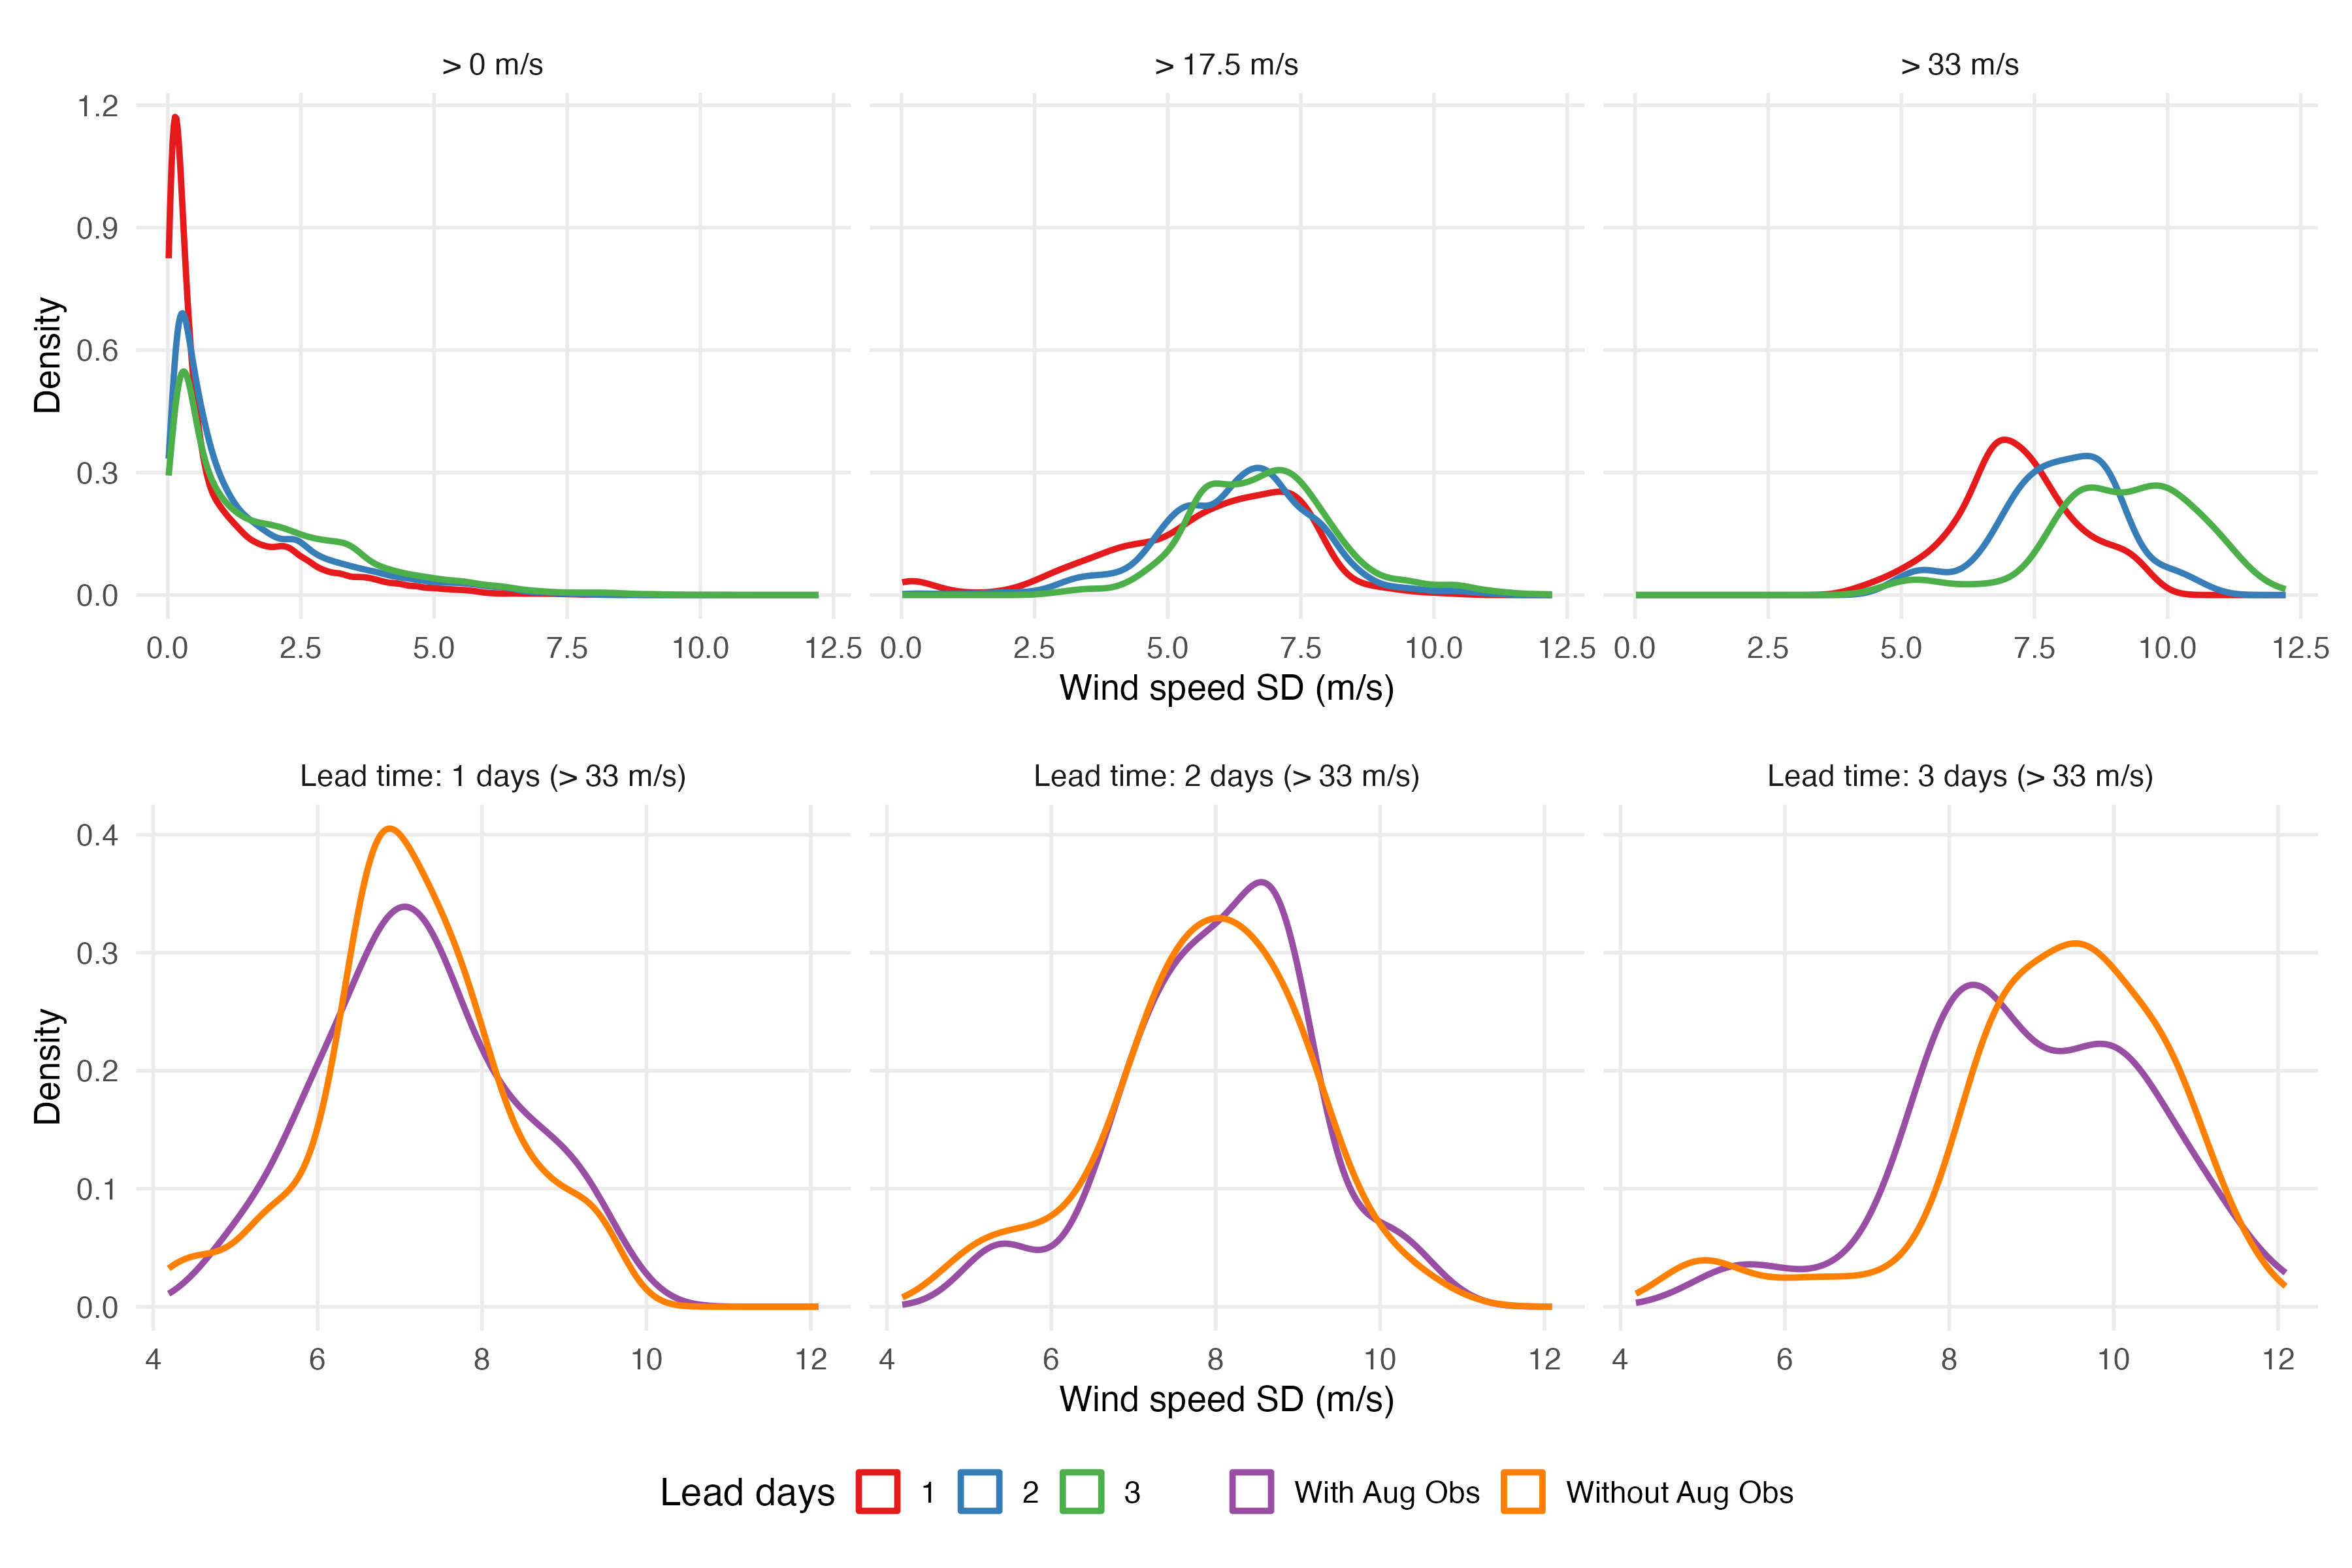
\includegraphics[width=1.0\textwidth]{figures and tables/augmented_panel.png}
    \caption{\textbf{Forecast Uncertainty Dynamics and the Impact of Augmented Observations.} \textit{Top Row:} Kernel density estimates of forecast wind speed ex-ante standard deviation ($\sigma$) by lead time (Red=1 day, Blue=2 days, Green=3 days), stratified by storm intensity. \textit{Bottom Row:} The specific impact on ex-ante standard deviation of augmented observations for hurricane-force winds ($>33$ m/s).}
    \label{fig:uncertainty_panels}
\end{figure}

The bottom row isolates the specific contribution of the observation network for these high-impact events. Comparing the distributions with (Purple) and without (Orange) augmented observations reveals a systematic reduction in forecast noise. At the critical 3-day lead time, the \emph{without augmented observations} distribution flattens and extends to the right, indicating a high probability of uncertainty (peaking around 9--10 m/s). In contrast, the assimilation of reconnaissance data shifts the distribution to the left (peaking around 8 m/s) and truncates the right tail. 

To formalize the visual pattern in Figure \ref{fig:uncertainty_panels}, we estimate a regression of forecast uncertainty ($\sigma$) on the presence of augmented observations. We restrict the sample to hurricane-force realizations ($>33$ m/s) at the critical 3-day lead time, and controlling for both observed wind, county-specific exposure, and unobserved storm heterogeneity. The analysis is presented in Table \ref{tab:noaa-controls}. Overall, we find that augmented observations reduce the forecast wind speed standard deviation by approximately 0.26 m/s (SE $\sim$ 0.10, $p < 0.01$). 

\begin{table}

\caption{Regression Analysis of the Effect of Augmented Observations in Ex-Ante Uncertainty \label{tab:noaa-controls}}
\centering
\begin{adjustbox}{max width = \textwidth}
\begin{threeparttable}
\begin{tabular}[t]{lcccc}
\toprule
  & (1) & (2) & (3) & (4)\\
\midrule
$\delta$: Augmented Observations & \num{-0.258}*** & \num{-0.258}*** & \num{-0.258}*** & \num{-0.258}***\\
 & (\num{0.093}) & (\num{0.095}) & (\num{0.094}) & (\num{0.096})\\
 &  &  &  & \\
Observations & 124 & 124 & 124 & 124\\
 &  &  &  & \\
Wind Controls &  &  & \checkmark & \checkmark\\
County FE & \checkmark & \checkmark & \checkmark & \checkmark\\
Hurricane FE &  & \checkmark &  & \checkmark\\
\bottomrule
\end{tabular}
\begin{tablenotes}
\item * p $<$ 0.1, ** p $<$ 0.05, *** p $<$ 0.01 Standard errors clustered at the county level. The sample is restricted to the 2017--2020 augmented-observations denial archive at the 3-day lead time and hurricane-force realizations ($\geq$ 33 m/s); Hurricane Maria is excluded because of its Puerto Rico landfall. The coefficient $\delta$ is the average reduction in the ex-ante wind-speed forecast standard deviation attributable to the assimilation of dropsonde profiles (the ALL configuration of \citet{DitchekEA2023}); the negative sign reflects that AO assimilation lowers ensemble spread relative to the no-dropsonde (NO) counterfactual. Wind Controls includes the realized wind speed (m/s) as a continuous covariate.
\end{tablenotes}
\end{threeparttable}
\end{adjustbox}
\end{table}


\subsection{Stage 3: Projecting Economic Gains}

In the final stage, we project the economic value of the observational improvements. Using the results from Stage 2, we found that augmented observations reduce the forecast standard deviation by approximately $\delta = 0.26$ m/s at the 3-day lead time. Because the cost function is convex in errors (quadratic), the monetary value of this reduction depends on the baseline level of uncertainty ($\bar{\sigma}$) characterizing the storm.\footnote{Recall that the value of a forecast improvement is proportional to the reduction in error variance: $\Delta \sigma^2 = \sigma^2_{No} - \sigma^2_{All} \approx 2\bar{\sigma}\delta$.}

With an average baseline forecast uncertainty ($\bar{\sigma}$) of approximately 8.98 m/s for the hurricanes in the sample, the 0.26 m/s physical improvement translates to a reduction in variance of roughly 4.7 (m/s)$^2$. Scaling this variance reduction by the marginal cost parameter ($\hat{\beta}^w_{Hurr} = 5.16$) yields an estimated benefit of augmented observations of approximately \$24 million per county per storm, for counties predicted to be exposed to hurricane-force winds. 

We can now directly derive the value of augmented observations. We note that for the storms with aircraft reconnaissance between 2017 and 2020, only 124 counties were predicted to experience hurricane-force wind speeds. This implies that the total retrospective social value of the augmented observations in this time period is approximately \$3 billion. 

\subsection{Cost-Benefit Analysis}

To contextualize our estimates, we perform a cost-benefit analysis comparing the program's benefits to its operational expenditures. Based on the FY25 Aircraft Rate, a standard hurricane reconnaissance mission typically involves the WP-3D Orion (P-3) or the G-IV Gulfstream (G-IV). A 9-hour P-3 mission costs approximately \$60,000 (\$6,446 per hour plus a \$1,964 daily rate), while a similar G-IV mission costs roughly \$45,000. 

Assuming a major hurricane requires an intensive deployment of ten such missions to maintain the observed 0.26 m/s precision gain at the 3-day lead time, the total flight expenditure per storm is approximately \$0.5 million. Comparing this to our estimated benefit of \textbf{\$25.77 million per affected county}, the return on investment (ROI) is substantial. Even if a storm impacts only a single hurricane-force county, the benefit-to-cost ratio is approximately 50-to-1. 

While federal recapitalization plans identify significant capital costs in replacing the aging P-3 fleet with C-130 platforms, the social value generated in just a few active hurricane seasons is sufficient to cover the entire cost of a new fleet several times over. The information provided by augmented observations represents an exceptionally high-leverage investment in national economic resilience.

\section{Policy Recommendations} \label{sec:policyrecs}

The findings of this study demonstrate that augmented observations provide a high-leverage economic return by reducing forecast uncertainty during high-intensity events. Based on the results documented here, and to ensure transparent evaluation of future capital investments, we propose the following four policy recommendations:

\paragraph{Institutionalization of Routine Data-Denial Studies.}
Currently, data-denial experiments are often conducted as isolated research exercises. We recommend the institutionalization of routine data-denial studies for \emph{all} landfalling hurricanes in the United States. By systematically running counterfactual models for every major event, NOAA can maintain a continuous, empirical record of the physical marginal contribution of dropsondes. This routine assessment would allow for the identification of specific storm environments where aircraft data are most impactful. We conjecture that this practice will also contribute to further optimizing flight patterns and deployment strategies.

\paragraph{Standardization of Performance Metrics.}
To bridge the gap between meteorological accuracy and economic preparedness, NOAA should implement simple, standardized performance metrics for data-denial assessment that explicitly measure both \textit{ex-ante} and \textit{ex-post} error. While \textit{ex-post} error is the traditional metric for meteorological verification, \textit{ex-ante} metrics---specifically the reduction in ensemble spread or forecast standard deviation---are the primary drivers of protective decision-making. Reporting the reduction in forecast variance ($\Delta \sigma^2$) alongside traditional error tracks would provide a more direct link to the socio-economic value generated by aircraft missions.

\paragraph{Unification of Economic Benefit Analysis.}
The justification for capital investments, such as the \textit{NOAA Aircraft Recapitalization Plan}, has historically relied on assumption-based scenarios and qualitative ``value chain'' arguments. We recommend a unification of benefit analysis based on the structural methodology presented in this study. By replacing hypothetical scenarios with a loss function tied to observed forecast precision gains, NOAA can provide a mathematically rigorous, evidence-based justification for the acquisition of new platforms, such as the C-130. This approach anchors the ``External Benefits'' in observed historical data rather than projected assumptions.

\paragraph{Dissemination and Routine Reporting.}
The methodology and results of these economic valuations should be disseminated broadly to stakeholders, including Congress, FEMA, and the broader meteorological community. We recommend the creation of a routine ``Socio-Economic Impact Report'' for the aerial reconnaissance program, updated on a biennial basis. Providing transparent, updated estimates of the per-county and per-storm ROI ensures that program funding remains commensurate with its multi-billion dollar contribution to national economic resilience.


%------------------------------------------%
%       Conclusion and Discussion
%------------------------------------------%

\section{Conclusion and Discussion} \label{sec:conclusion}

This study provides a novel empirical valuation of augmented aircraft observations in the context of hurricane forecasting. By linking data denial experiments to a structural model of hurricane costs, we quantify the socio-economic return on in-situ meteorological data collection. Our results demonstrate that the assimilation of dropsonde data from the NOAA aircraft fleet significantly improves forecast precision, which in turn generates substantial social value by reducing both avoidable damages and misallocated protective expenditures.

Our analysis proceeds in three stages. First, we establish that the social cost of forecast uncertainty is highly sensitive to intensity, with a marginal cost parameter that is statistically significant only for hurricane-force events. Second, we show that augmented observations reduce forecast standard deviation by approximately 0.26 m/s at the critical 3-day lead time. Finally, we project these physical gains into monetary terms. 

With a baseline forecast uncertainty of approximately 8.98 m/s for counties predicted to experience to hurricane-force winds, the 0.26 m/s prediction  improvement translates into a benefit of approximately \$25.77 million per county per storm. The cost-benefit implications of these findings are stark. Based on FY25 aircraft rate tables, the operational cost of a standard reconnaissance mission is approximately \$40,000 to \$60,000. Even with an intensive deployment of ten missions per storm, the total flight cost ($\approx$\$0.5 million) is outweighed by the benefits generated for a single affected county by a factor of 50. Aggregated across our 2017--2020 estimation sample, the total retrospective social value reaches \$3.2 billion, suggesting a return on investment that far exceeds the cost of flight hours.

These results provide a bottom line for the strategic recapitalization of the NOAA aircraft fleet. While the \textit{2022 NOAA Aircraft Plan} identifies significant capital requirements for replacing aging platforms like the WP-3D with newer C-130 aircraft, our findings suggest that these investments are highly cost-effective. The social value generated in just a few active hurricane seasons is likely sufficient to cover the entire cost of fleet replacement. 

However, our estimates likely represent a lower bound. Our framework focuses on wind-speed-driven costs and does not explicitly account for the value of improved precipitation or storm surge forecasts, nor does it capture secondary benefits to the maritime and aviation sectors identified in NOAA’s external benefit reports. Future research should aim to integrate these multi-hazard dimensions to provide an even more comprehensive account of the value of weather information. Ultimately, this study underscores that in the face of increasing hurricane intensity and coastal exposure, the information provided by augmented observations is one of the most high-leverage tools available for enhancing national economic resilience.


%------------------------------------------%
%                References
%------------------------------------------%
\FloatBarrier
\newpage
\begin{singlespace}
\bibliographystyle{references/econ}
\bibliography{references/references}{}
\end{singlespace}
%------------------------------------------%
%                Appendix
%------------------------------------------%
\FloatBarrier
\newpage
\appendix
\begin{Large}
\section{Appendix}
\end{Large}

% Reset figure/table #'s
\setcounter{table}{0}
% Add an A in front of tables and figures
\renewcommand{\thetable}{A\arabic{table}}

\begin{appendices}
\end{appendices}

\end{document}
